\section{Case study}

To show the functionality and applicability of the automatic domain decomposition library a few case studies were carried out.
This chapter and the following sections will outline each case study and the corresponding experimental results.

\subsection{Case 1: Burger's equation}
Burger's equation is a well-known nonlinear partial differential equation.
It is widely used to test numerical schemes since it has analytical solutions for a set of initial conditions.
Burger's equation can be used to model various physical phenomena.
Most commonly it is used as a model for traffic flow or shock waves in a fluid.

\subsubsection{Case description}

The two-dimensional, viscid Burger's equation is given by the following system of equations as described in \citet{zhao2011new}:

\begin{equation}
\begin{split}
\pdv{u}{t} + u \pdv{u}{x} + v \pdv{u}{y} = \varepsilon \left( \pdv{^2 u}{x^2} + \pdv{^2 u}{y^2} \right) \\
\pdv{v}{t} + u \pdv{v}{x} + v \pdv{v}{y} = \varepsilon \left( \pdv{^2 v}{x^2} + \pdv{^2 v}{y^2} \right) \\
\text{with } \left(x, y, t\right) \in D \times \left(0,T\right]
\end{split}
\end{equation}

The initial and boundary conditions are generally described by the following equations:

\begin{equation}
\begin{split}
\text{Initial conditions: } \\
u\left(x, y, 0\right) = u_0\left(x, y\right), \left(x, y\right) \in D \\
v\left(x, y, 0\right) = v_0\left(x, y\right), \left(x, y\right) \in D \\
\text{Boundary conditions: } \\
u\left(x, y, t\right) = f\left(x, y, t\right), \left(x, y, t\right) \in \partial D \times \left(0, T\right] \\
v\left(x, y, t\right) = g\left(x, y, t\right), \left(x, y, t\right) \in \partial D \times \left(0, T\right]
\end{split}
\end{equation}

% TODO FOOTNOTE CHECK CORRECT NUMBERING

The first set of initial and boundary conditions are the ones used by Shankar. \footnote{https://ch.mathworks.com/matlabcentral/fileexchange/38087-burgers-equation-in-1d-and-2d}

The following equations describe the Shankar test case fully and fig. \ref{fig:shankar_ic1} and fig. \ref{fig:shankar_ic2} visualizes the initial condition.

\begin{equation}
\begin{split}
\text{Domain: } \\
D = \left(0,2\right) \cross \left(0,2\right) \\
T = \left(0, 0.6\right]
\text{Initial conditions: } \\
u_0\left(x, y\right), \left(x, y\right) = \begin{cases}
0, \text{ in } \left(0.5, 1.0\right) \times \left(0.5, 1.0\right) \\
1, \text{otherwise}
\end{cases}
\\
v_0\left(x, y\right), \left(x, y\right) =  \begin{cases}
1, \text{ in } \left(0.5, 1.0\right) \times \left(0.5, 1.0\right) \\
0, \text{otherwise}
\end{cases}
\\
\text{Boundary conditions: } \\
f\left(x, y, t\right), \left(x, y, t\right) = 0 \\
g\left(x, y, t\right), \left(x, y, t\right) = 0 \\
\text{Other parameters: } \\
\text{Viscosity: } \varepsilon = 0.01
\end{split}
\end{equation}

\begin{figure}
\centering
\begin{subfigure}{.5\textwidth}
  \centering
  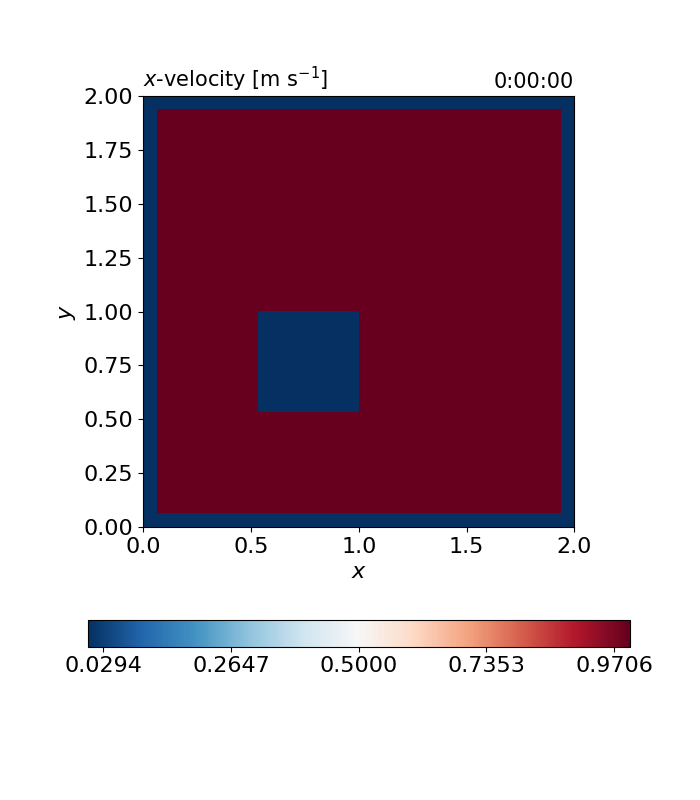
\includegraphics[width=1.1\linewidth]{test_shankar_forward_backward_field_u_at_0.png}
  \caption{X-velocity initial condition.}
  \label{fig:shankar_ic1}
\end{subfigure}%
\begin{subfigure}{.5\textwidth}
  \centering
  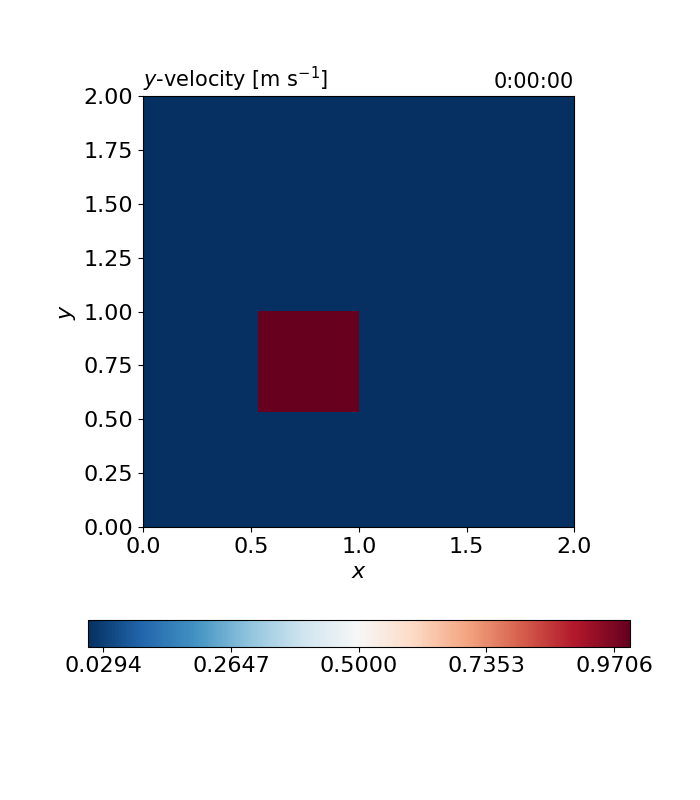
\includegraphics[width=1.1\linewidth]{test_shankar_forward_backward_field_v_at_0.png}
  \caption{Y-Velocity initial condition.}
  \label{fig:shankar_ic2}
\end{subfigure}
\caption{Initial condition for the Shankar test case.}
\label{fig:shankar_ic}
\end{figure}

\paragraph*{}

The second set of initial and boundary conditions are the same as used in \citet{zhao2011new}:

\begin{equation}
\begin{split}
\text{Domain: } \\
D = \left(0,2\right) \cross \left(0,2\right) \\
T = \left(0, 0.6\right]
\text{Initial conditions: } \\
u_0\left(x, y\right), \left(x, y\right) = \begin{cases}
0, \text{ in } \left(0.5, 1.0\right) \times \left(0.5, 1.0\right) \\
1, \text{otherwise}
\end{cases}
\\
v_0\left(x, y\right), \left(x, y\right) =  \begin{cases}
1, \text{ in } \left(0.5, 1.0\right) \times \left(0.5, 1.0\right) \\
0, \text{otherwise}
\end{cases}
\\
\text{Boundary conditions: } \\
f\left(x, y, t\right), \left(x, y, t\right) = 0 \\
g\left(x, y, t\right), \left(x, y, t\right) = 0 \\
\text{Other parameters: } \\
\text{Viscosity: } \varepsilon = 0.01
\end{split}
\end{equation}

\begin{figure}
\centering
\begin{subfigure}{.5\textwidth}
  \centering
  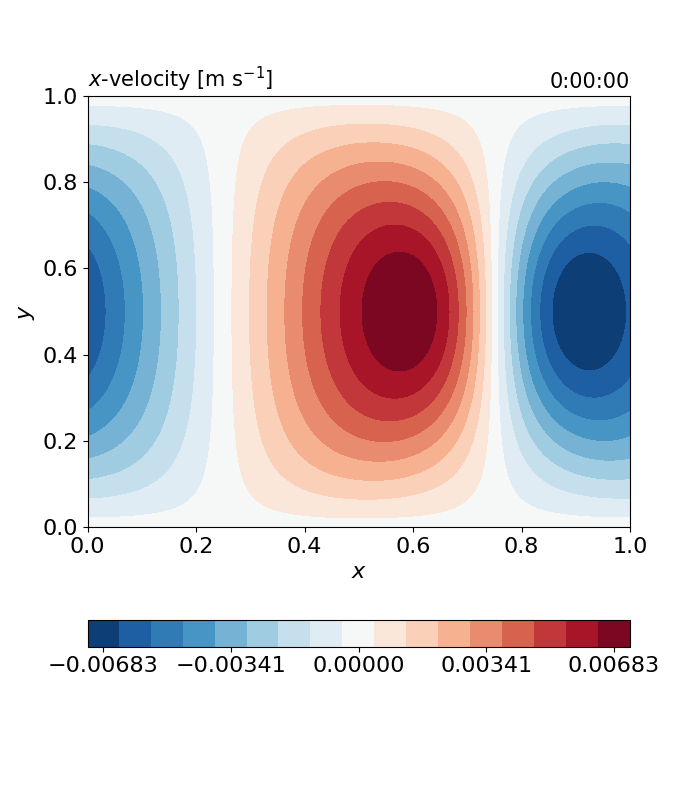
\includegraphics[width=1.1\linewidth]{test_zhao_forward_backward_field_u_at_0.png}
  \caption{X-velocity initial condition.}
  \label{fig:zhao_ic1}
\end{subfigure}%
\begin{subfigure}{.5\textwidth}
  \centering
  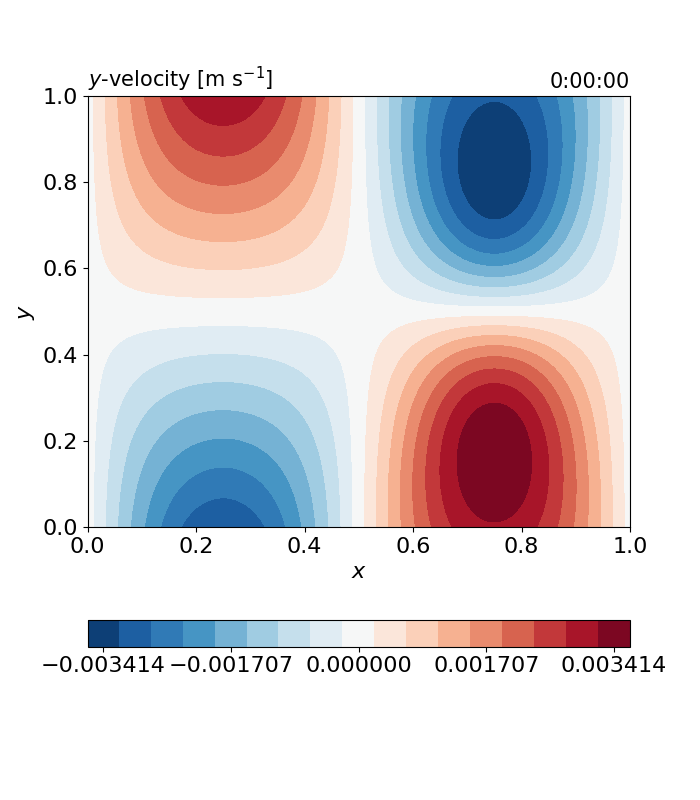
\includegraphics[width=1.1\linewidth]{test_zhao_forward_backward_field_v_at_0.png}
  \caption{Y-Velocity initial condition.}
  \label{fig:zhao_ic2}
\end{subfigure}
\caption{Initial condition for the Zhao test case.}
\label{fig:zhao_ic}
\end{figure}

\paragraph*{}

\subsubsection{Implementation details}

\subsubsection{Experimental setup}

\subsubsection{Experimental results}


\subsection{Case 2: Shallow water equation}

\subsubsection{Case description}

\subsubsection{Implementation details}

\subsubsection{Experimental setup}

\subsubsection{Experimental results}
